\documentclass[titlepage]{article}
\usepackage{amsmath}
\usepackage{enumerate}
\usepackage{listings}
\usepackage{graphicx}
\title{CS 180 Homework 5}
\author{Robert Geil \\
University of California, Los Angeles
}
\lstset{frame=tb,
  showstringspaces=false,
  columns=flexible,
  basicstyle={\small\ttfamily},
  breaklines=true,
  tabsize=2
}
\numberwithin{equation}{subsection}
\begin{document}
\maketitle

\section{Closest Pair of Points}
\subsection{Problem}
Given a set of $n$ points on a plane, find the closest pair of points, defined by the euclidian distance
between the two
\subsection{Algorithm}
\begin{lstlisting}
1. Sort the input based on x coordinates
2. Split into subgroups of size 2, take the distance between these two to be the shortest
3. For each pair of neighboring subgroups, it must be true that the shortest pair is either the shortest pair on the left, or the shortest pair on the right or a pair containing a single point on left and right
4. Take the minimum of the distances on the left and the right as a value d
5. For each element on the left within that distance d from the split, examine all points on the other side that are also within d in the x direction and either -d or d away from the y coordinate. Save the minimum
6. Take the minimum of the value on the left, the right, and the middle values examined. Set that to be the new min and merge the left and right together
7. If there are still multiple partitions, go to step 3
\end{lstlisting}
\subsection{Proof}
We will prove the correctness by induction. First, for the base case, it is trivially true that for a group of
two points, the shortest path is between those two points, as no other pairing is possible. Inductively, for two
neighboring sets of points, it must be true that the shortest pair is either the shortest pair on the left, or
the shortest pair on the right, or a pair of points where one exists on the left and one on the right. We can see
this is true, as this forms an exhaustive search of all possible points. Finally, we prove that our trick of
only looking at points a distance\textit{delta} from the divide doesn't reject shorter pairs. \textit{delta} is the minimum of the
shortest distances on the left and right. If we look at a pairing of any element on the left (without loss of 
generality) with one on the right, where the left side is more than \textit{delta} away, the distance from left to the 
divide will already be \textit{delta}, and as such the total distance must be \textit{delta} or more. As we already have a pair
satisfying a distance of \textit{delta}, this won't produce a shorter path. Likewise when observing the values above and
below (in the Y direction), we can restrict our search space with the same logic. Any value more than \textit{delta} 
away in the Y direction must already be greater than the min of the shortest distance on the left and right.
Therefore we prove by induction that this algorithm will always find the shortest pair of points.
\subsection{Runtime}
Overall the runtime of this algorithm is O($n\log n$). Initially we perform a sort based on x axis, which takes
O($n\log n$) time. After that, we see that there is a process of dividing and joining into subgroups. Because 
each subgroup is split and joined in a binary fashion, with the same logic as Merge Sort, we see that there 
are O($\log n$) of these join operations. As for the time complexity of each individual operation, we can prove that
each step is done in linear time. Comparing the two existing shortest values on the left and right takes constant
time. To find the pairing across the divide, it would naievely appear that it takes O($n^{2}$) time. However, using
clever constraints, we can reduce this to linear time. First, we select each point on the left that is within
a distance \textit{delta} of the divide. Note this may be O($n$) elements. For each of these, we need only examine
those a distance \textit{delta} from the side, and a distance \textit{delta} above and below the Y coordinate, as
proven above. While this may seem to take linear time to the number of points on the right, we can prove it is
a constant time operation. We claim there are at most a constant number points on the left that must be tested. 
Within the bounding box of \textit{delta} on X and \textit{delta} on Y, the sides can be divided to form grids
that are \textit{delta}/2 by \textit{delta}/2 in size, of which there will be 8. By the pigeonhole principle,
there cannot be more than 1 point within any one of these given boxes. By contradiction, if there were two points
within one box, they would have to be closer than \textit{delta} apart, and would therefore be the shortest on the
right, violating our earlier assumption that \textit{delta} is the shortest distance on the right and left individually.
Therefore, we prove we must only examine a constant number of elements for each element on the left. The searching
of these bounding boxes can be cleverly done with a pre-sorting, by additionally sorting the Y axis points, another
O($n\log n$) task at the beginning. This means each step in the merging takes O($n$) time. Combined over all the
merge steps, we prove we have a final time complexity of O($n\log n$).

\section{Longest Path in Ordered Graph}
\subsection{Problem}
An ordered graph is a DAG such that there is a distinct ordering of nodes by index. Each edge only goes
from a node of a lower index to one of a higher index, and every node besides the last has at least one
edge originating from it. Find the longest path in terms of segment count from node $v_0$ to $v_n$.
\subsection{A Bad Approach}
The provided algorithm is a greedy approach to solving the problem, and it fails under certain situations.
For example, if the first step can pick a nearby value, this will always be added to the solution. However,
due to the greedy nature of the algorithm this may pigeonhole the solution to including a poor choice which
may then jump directly to the end. 
\begin{figure}
    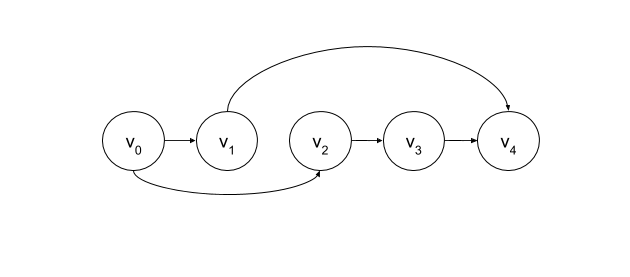
\includegraphics[width=\linewidth]{counter2.png}
    \figurename{: Greedy Counter Example}
\end{figure}
\\
In the above figure, the greedy algorithm would select the path ($v_0$, $v_1$, $v_4$), for a total length of
2 segments. However, the optimal solution is ($v_0$, $v_2$, $v_3$, $v_4$) for a total length of 3 segments.
\subsection{Correct Algorithm}
This solution will use a dynamic programming paradigm, each time building up the solution inductively. This
solution relies on the nodes being processed in order (ie $v_0$, $v_1$, \dots $v_n$)
\begin{lstlisting}
1. Set a length of each node, initially set to zero
2. Select a current node i initially set to the first value V(0)
3. For each incoming edge (from node k to i) on i, if length(k) + 1 > length(i), set length(i) = length(k) + 1
4. If the last node processed was the last value in the graph, return length(V(i))
5. Set the current node to V(i+1) and go to step 3
\end{lstlisting}
\subsection{Proof}
This proof relies on an exhaustive search, but in an ordered fashion, and can be proven by induction. For the
base case, trivially prove that the longest path to $v_0$ is length zero, as there are no earlier nodes which
could contribute to a path. For each remaining node $v_i$ in the graph, we can see that the longest path to that
specific node must come from the longest path to one of the earlier nodes $v_j$ where $j < i$. Since the longest
path must come from one of these, as there are no other inputs to $v_i$, we can maximize the path to $v_i$ by
selecting the simple longest path among the longest paths for the input nodes, and adding one. As such, we prove
that this algorithm will find the longest path to an arbitrary node $v_i$. By extension, taking $i = n$, this
will give a solution for the longest path to $v_n$.
\subsection{Runtime}
This algorithm has a similar runtime to many graph traversal algorithms. We see that for each node from 0 to $n$,
we examine all the incoming edges to the node. Since an edge can only be incoming to exactly one node, each edge is
looked at at most once, giving us a complexity of O($e$). At each of these edges, a constant amount of work is
done (a comparison or two), so we have a contribution of just O($e$). In addition, each node is visited initally
to set values for longest path to zero, so our overall time complexity is O($n+e$). With this problem, along with most
dynamic programming problems, we should consider space usage as well. For this, we have a space complexity of O($n$).
Each node must only store the longest distance to that node, and this recurrance is required to calculate further
nodes, so it cannot be discarded. Therefore our overall runtime of O($n+e$) and space is O($n$).

\section{Word Segmentation}
\subsection{Problem}
%TODO: Review this, it probably sucks...
For some languages, there isn't a special character to denote a word break, and as such, multiple words may
appear next to each other. Within these languages, it is necessary to determine where the words should break
up, as different splits may be more correct ways of dealing with the given set of characters. For example,
\textit{hellothere} could be represented as the correct \textit{hello there} or \textit{hell other e} or 
\textit{hel loth ere} or any other combination. Assuming we can assign a "quality" factor to a series of letters
depending on how much of a word it is (such as quality(\textit{hello} = 5, while quality(\textit{e}) = -2)),
provide an algorithm that finds the highest quality splitting of an input.
\subsection{Algorithm}
This dynamic programming problem can be solved using a recurrence relationship, examining the optimal solution
for 0 to $n$ letters and 0 to $n$ words.
\begin{lstlisting}
1. Create an NxN table, with columns the number of letters and rows the number of words and values are quality
2. Begin with an output containing just the first character of the input
3. For each additional letter, it is either part of the last word, or a new word
4. Set the current table entry to max(table[row - 1, col - 1] + quality(new char), table[row, col - last word length] + quality(last word + new char)), and a pointer back to the selected node, go to step 3
5. Search down the rightmost column for the maximum value, traversing pointers backwards will reveal the highest quality breakdown
\end{lstlisting}
\subsection{Proof}
This algorithm is true by induction. We see that for the base case of an input of length 1, it must be that the
one element is in a single word, and that word is in the result. From there, each additional character is either in
the last word available, or is the start of a new word. If it is the start of a new word, the quality must be
the quality of the previous optimal solution plus the quality of the new character. If the new character is
part of the last word, then the quality of the solution is the quality of the optimal solution with the first $j$
words plus quality($j+1$st word + last character). As we can see here, both the options for every additional character
are explored, so when taking the maximum of the divides of all the characters, all possible solutions have been explored,
so our solutions is proven correct.
\subsection{Runtime}
In this solution, we are iterating over an $n*n$ matrix. At each node, we perform a constant amount of work, with the
assumption that our \textit{quality} operation is performed in a constant amount of time. At the end, we find the maximum
of the rightmost column, which takes $n$ steps, and traverse back through the matrix, again hitting at most $n$ nodes.
Therefore, we see that we have an overall time complexity of O($n^2$). In addition, we use O($n^2$) space, as the
array storing all the intermediary values has dimension $n*n$.

\section{Supercomputer Selection}
\subsection{Problem}
You have two supercomputers which can be used to perform calculations for a project. However, each can only perform
a given number of operations in a minute, and that value varies depending on the load on the machine. The project can
be switched from machine to machine, but requires a minute of no operations to perform the swap. Find an algorithm
that generates the swapping and compute ordering that maximizes the number of cycles used on the machine.
\subsection{A Bad Approach}
While it may initially seem that a greedy approach would work on the problem, a quick counter example shows that
solution cannot work. In the greedy approach, if the value of $a_i + a_{i+1} < b_{i+1}$, a swap is done. However,
with the following, that solution won't work out. 
\begin{center}
  \begin{tabular}{|c|c|c|c|c|}
    \hline
  Computer & Minute 1 & Minute 2 & Minute 3 & Minute 4\\ \hline
  A & 6 & 1 & 1 & 50 \\
  B & 5 & 5 & 5 & 5  \\
  \hline
  \end{tabular}
\end{center}
The greedy algorithm will select A to begin, and then switch at time 2, since $a_2 + a_3 < b_3$. However, performing
the switch will place on computer B. Looking ahead from Minute 3, the algorithm will instead see that $b_3 + b_4 < a_4$
and will then switch back to A. Overall, the sequence will be (A, switch, switch, A), giving a value of 56. However,
an optimal solution would produce (B, B, switch, A) which provides a value of 60, improving on the greedly algorithm.
\subsection{A Good Algorithm}
%TODO
\section{Rod Division}
\subsection{Problem}
Given a rod of length $n$, and a set of prices for smaller pieces of the rod, determine the maximum value that can be obtained
by cutting the rod up and selling the pieces.
\subsection{Algorithm}
This problem can be solved using a dynamic programming model, where the parameters are the length of the rod, and the segments being sold.
\begin{lstlisting}
1. Create an n*m matrix with n columns labeled 1 to n, for the length of the rod, and m rows for the m sale pieces, such that the first entry contains 1 (arbitrary) sale piece, and the mth contains all of them.
2. Proceeding in row-major order, examine the ith row and the jth column 
3. Find the optimal solution as max(the ith sale piece price + optimal[i, j - size of sale piece], or optimal[i - 1, j]). If j is less than the size the first option is simply optimal[i, j-1], and if i = 0, the second option is just 0
4. Go back to step 2 until the last square is filled in
5. The value in the lower right grid piece is the optimal value
\end{lstlisting}
\subsection{Proof}
This proof can be shown inductively. The base case, where there are no elements to sell and the rod length is zero gives us a trivial solution of
zero for the maximum profit. Inductively, for a given segment and a given size, the segment is either in the solution, taking up $k$ length, or is
not in the solution. In the first case, the optimal solution is the optimal solution for a rod of length $j-k$ plus the value of the segment,
while in the second case, the optimal solution is the optimal solution for a rod of length $j$ without the segment in question. As our algorithm examines both of these
possibilities and selects the maximum of the two, it is impossible for a rod of length $n$ and possible element set with the given segment
to be more valuable than what our algorithm selects. As such, since at the lower left of the grid we produce the optimal solution with
all possible segments and a full length rod of length $n$, that solution must be optimal.
\subsection{Runtime}
The runtime of this algorithm is O($n*|e|$), where $|e|$ is the number of segment/price values, and $n$ is the length of the rod. Since we
are computing each element in the grid, and the grid has $n$ columns, and $|e|$ rows (where each row adds a segment/price value), and for each
element, we are performing a constant number of operations, finding the max of two values and looking backwards, to build the grid takes O($n*|e|$)
time. For space, since we must maintain both the current row and previous row in memory (as we may reference row $i-1$ and values $j-k$ in the
current row), we have a space complexity of the size of a row, which is O($n$), where $n$ is the length of the rod.

\section{Coin Game}
\subsection{Problem}
Given an array of $n$ coins, each with a value and where $n$ is even, two players can take turns removing a coin from either end.
The total score is the sum of all the values of coins that a given player has removed. Determine an algorithm that maximizes the
earnings of the player who moves first.
\subsection{Algorithm}
This algorithm relies on dynamically programming the value of each possible sub-interval. Since there are two players, this is a bit more
of a complex issue. For every arbitrary pairing, the player needs to pick either left or right ($i$ or $j$), where the choice maximizes
the value of input[choice] + input[interval after your opponent moves]
\begin{lstlisting}
1. Create an NxN matrix M where columns represent lower bound (values from 0 to n-1) and rows represent the upper bound (values from 0 to n-1). The values are a score and a pointer to another grid cell
2. Proceed through in row-major order from column i in (O, n) and row j in (0, n). 
3. If i > j, continue. If i == j, set M[i, j] = input[i], if i + 1 == j, set M[i, j] = max(input[i], input[j])
4. If nothing above matched, let l = input[i] + value of pointer of M[i+1, j]. Let r = input[j] + value of pointer of M[i, j-1].
5. Set M[i, j] to be the max of l and r, and set the pointer to point to M[i+1, j] if l was greater, and M[i, j-1] if r was greater.
6. Continue while there are empty squares
7. Return the value at square M[0, n]
\end{lstlisting}
\subsection{Proof}
This solution can be proved inductively, as it is an exhaustive search of the possible space. For each arbitrary sub-interval between $i$ and $j$
at the lower and upper bounds respectively, the player can either select $i$ or $j$ to remove. Since, through our grid, all possible intervals
are examined, we prove that each possible interval will be examined. For the proof of optimality, we turn to induction. For the base case,
we can see through inspection that when one element remains, the optimal choice is to select that one element, and when there are two elements,
the optimal choice is to select the larger of the two. For the inductive step, we see that the player can either select the left value, or 
the right value. For either of these, we assume that there is some optimal choice for the one-smaller problem, by induction. Further, from
that one-smaller value, there is again a smaller value (as saved by the pointer to previous within our solution). Therefore, the sum of
the selected value plus the optimal value of two earlier is the expected score by making that move. Since all players move optimally, we
see that this will generate an optimal solution for the $k$th step, proving our induction.
\subsection{Runtime}
The runtime of this algorithm if O($n^2$). For the main body of the algorithm, we iterate over every possible sub-interval. Because
there are $n\choose 2$ ways to pick two end points of an interval out, and ${n \choose 2} \approx n^2$, there are O($n^2$) optimal sub-intervals.
In order to calculate each of these, we perform a constant set of operations (doing a few comparisons and lookups in the grid of pre-computed values).
Therefore, our overall runtime remains O($n^2$).
\end{document}